\documentclass[10pt]{beamer}

\usepackage[spanish]{babel}
\usepackage{fontspec}
\usepackage{tikz}
\usetikzlibrary{arrows.meta,positioning,shapes.geometric,fit,calc}
\usepackage{booktabs}
\usepackage{tabularx}
\usepackage{listings}
\usepackage{amsmath}
\graphicspath{{./imagenes/}}


% Colores institucionales ESPE para el tema Beamer
\definecolor{espeGreen}{HTML}{0F3D2E}
\definecolor{deepTeal}{HTML}{123C55}
\definecolor{softGold}{HTML}{C6A24A}
\definecolor{ink}{HTML}{1F2933}
\definecolor{mist}{HTML}{EFF3F1}
\definecolor{cloud}{HTML}{F8FAF8}
\definecolor{accentRed}{HTML}{B44B3F}
\definecolor{steel}{HTML}{44546A}
\definecolor{fog}{HTML}{DCE2DE}


% Configuración del tema Beamer (Madrid/similar adaptado)
\usetheme{Madrid}
\usecolortheme{default}

% Aplicar colores personalizados a los elementos de Beamer
\setbeamercolor{structure}{fg=espeGreen}
\setbeamercolor{palette primary}{bg=espeGreen,fg=white}
\setbeamercolor{palette secondary}{bg=deepTeal,fg=white}
\setbeamercolor{palette tertiary}{bg=softGold,fg=ink}
\setbeamercolor{titlelike}{parent=palette primary,fg=white}
\setbeamercolor{block title}{bg=deepTeal,fg=white}
\setbeamercolor{block body}{bg=mist,fg=ink}
\setbeamercolor{normal text}{fg=ink,bg=white}

% Configuración del pie de página
\setbeamertemplate{footline}[frame number]
\setbeamertemplate{navigation symbols}{} % Quitar barra de navegación

\title[SentinelML-ABAC]{SentinelML-ABAC: Sistema de Control de Acceso Industrial Resiliente a Ataques de Evasión}
\subtitle{Ingeniería de Seguridad de Software}
\author[Grupo 1]{Caetano Flores, Jordan Guamán, Mesías Mariscal,\\Anthony Morales, Leonardo Narváez, Denise Rea}
\institute[ESPE]{Universidad de las Fuerzas Armadas ESPE}
\date[Julio 2026]{19 de julio de 2026}

% Configuración para listados de código
\lstset{
  backgroundcolor=\color{cloud},
  basicstyle=\ttfamily\tiny\color{ink},
  keywordstyle=\bfseries\color{deepTeal},
  commentstyle=\color{espeGreen!80!black}\itshape,
  stringstyle=\color{accentRed},
  frame=single,
  rulecolor=\color{espeGreen!30},
  tabsize=2,
  breaklines=true,
  showstringspaces=false
}

\begin{document}

% 1. Diapositiva de Título
\begin{frame}[plain]
  \titlepage
  \centering
  \vspace{-0.4cm}
  
\includegraphics[width=3.2cm]{espe.jpg}
  % Nota: Buenas tardes estimado docente y compañeros. Hoy presentaremos nuestro proyecto integrador de fin de parcial, enfocado en solucionar de forma novedosa las vulnerabilidades de la IA en control de acceso industrial.
\end{frame}

% 2. Tabla de Contenidos
\begin{frame}{Agenda del Proyecto}
  \centering
  \vspace{0.2cm}
  \begin{columns}[t, onlytextwidth]
    \begin{column}{0.54\textwidth}
      \large
      \tableofcontents[sections={1-3}, hideallsubsections]
    \end{column}
    \hfill
    \begin{column}{0.42\textwidth}
      \large
      \tableofcontents[sections={4-6}, hideallsubsections]
    \end{column}
  \end{columns}
  % Nota: Esta es la agenda que guiaremos el dia de hoy, abarcando desde la motivacion del problema, el sustento teorico del semestre, el detalle de la solucion novedosa y sus consideraciones de gobernanza.
\end{frame}

\section{Problema y Motivación}
\subsection{Problema y Motivación}

% 3. Problema y Motivación
\begin{frame}{El Desafío de la Convergencia IT/OT y la IA}
  \small
  \begin{columns}[onlytextwidth]
    \begin{column}{0.58\textwidth}
      \begin{block}{Entorno Industrial Crítico}
        Los sistemas SCADA y sensores IIoT se conectan mediante APIs analizadas por modelos de clasificación probabilística inteligentes.
      \end{block}
      \begin{block}{La Nueva Amenaza: Evasión Adversaria (FGSM)}
        \begin{itemize}
          \item Atacantes APTs inyectan ruido matemático imperceptible.
          \item Engañan al modelo haciendo pasar ataques como datos legítimos.
          \item Se elude la alerta del IDS y se sabotean los actuadores.
        \end{itemize}
      \end{block}
    \end{column}
    \hfill
    \begin{column}{0.38\textwidth}
      \centering
      
\includegraphics[width=0.95\textwidth]{scada_security.png}
    \end{column}
  \end{columns}
  % Nota: Los sistemas SCADA ya no están aislados. La integración de IA para clasificar anomalías introduce la vulnerabilidad de ejemplos adversarios (como FGSM), permitiendo sabotear físicamente la planta sin alarmas del IDS tradicional.
\end{frame}

\section{Marco Teórico Integrador}
\subsection{Marco Teórico Integrador}

% 4. Marco Teórico I: Ciberseguridad Tradicional
\begin{frame}{Fundamentos Criptográficos y de Control de Acceso}
  \begin{columns}[t, onlytextwidth]
    \begin{column}{0.48\textwidth}
      \begin{block}{Unidad 1 y 2: Fundamentos}
        \begin{itemize}
          \item \textbf{Tríada CIA}: Disponibilidad e integridad críticas en entornos OT.
          \item \textbf{Malware y Redes}: Botnets (ej., Mirai), rootkits, ataques MITM y replay.
          \item \textbf{Criptografía}: Cifrado híbrido (AES-256 para datos, ECC para firmas).
        \end{itemize}
      \end{block}
    \end{column}
    \hfill
    \begin{column}{0.48\textwidth}
      \begin{block}{Unidad 2 y 3: Protocolos}
        \begin{itemize}
          \item \textbf{Control de Acceso}: ABAC dinámico superando el RBAC estático.
          \item \textbf{Modelo Biba}: Integridad (*no-read-down, no-write-up*) para detener flujos de baja confianza.
          \item \textbf{Kerberos}: Autenticación centralizada por tickets, mitigando ataques Needham-Schroeder.
        \end{itemize}
      \end{block}
    \end{column}
  \end{columns}
  % Nota: Resumimos el contenido del semestre: combinamos criptografía híbrida y Kerberos para identidad, control ABAC con la estricta regla de integridad Biba, y mitigación de red industrial perimetral.
\end{frame}

% 5. Marco Teórico II: Seguridad en IA y MLSecOps
\begin{frame}{Seguridad de Modelos de ML en Producción}
  \small
  \begin{columns}[onlytextwidth]
    \begin{column}{0.58\textwidth}
      \begin{block}{Vulnerabilidad Probabilística}
        Los modelos sufren de envenenamiento de datos en el entrenamiento y evasión (FGSM) en inferencia. Las APIs LLM sufren jailbreaks y fuga de información sensible.
      \end{block}
      \begin{block}{Ciclo MLSecOps y NIST AI RMF}
        \begin{itemize}
          \item \textbf{Firma de Pesos}: Validar hashes SHA-256 en PKI antes de montarlos.
          \item \textbf{Safetensors}: Evitar RCE en deserialización de Pickles.
          \item \textbf{Drift}: Monitoreo de desalineación ($PSI$ y Wasserstein) para rollbacks rápidos.
        \end{itemize}
      \end{block}
    \end{column}
    \hfill
    \begin{column}{0.38\textwidth}
      \centering
      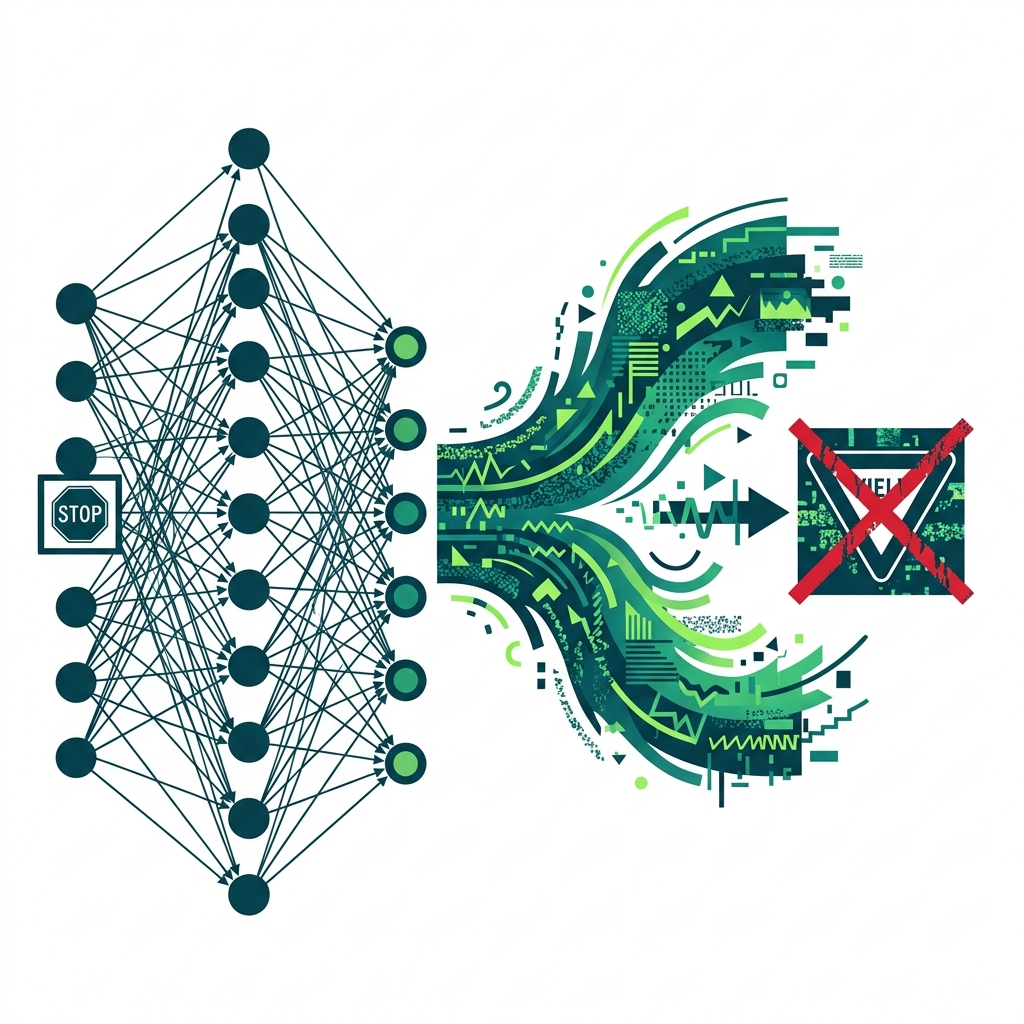
\includegraphics[width=0.95\textwidth]{adversarial_attack.png}
    \end{column}
  \end{columns}
  % Nota: Los modelos son dinámicos y exigen un flujo MLSecOps. Usamos Safetensors para evitar ejecución remota de código en deserialización y la Distancia de Wasserstein para monitorear anomalías estadísticas.
\end{frame}

\section{Solución Propuesta: SentinelML-ABAC}
\subsection{Solución Propuesta: SentinelML-ABAC}

% 6. Solución Propuesta
\begin{frame}{SentinelML-ABAC: Defensa Holística por Diseño}
  \small
  \begin{columns}[onlytextwidth]
    \begin{column}{0.58\textwidth}
      El tráfico pasa por tres compuertas lógicas antes de autorizar comandos físicos en la planta:
      \vspace{0.2cm}
      \begin{enumerate}
        \item \textbf{Criptográfica}: Tickets Kerberos y ECC para evitar suplantación y replay.
        \item \textbf{Preprocesamiento}: Suavizado y ruido gaussiano para mitigar perturbaciones FGSM.
        \item \textbf{Inferencia}: Safetensors sandboxed y control de acceso ABAC con integridad Biba.
      \end{enumerate}
    \end{column}
    \hfill
    \begin{column}{0.38\textwidth}
      \centering
      
\includegraphics[width=\textwidth]{secure_gate.png}
    \end{column}
  \end{columns}
  % Nota: SentinelML-ABAC integra tres filtros sucesivos: identidad mediante Kerberos, suavizado para invalidar ataques de gradiente adversarial y el motor ABAC que evalúa políticas bajo el rigor de integridad Biba.
\end{frame}

% 7. Arquitectura Técnica
\begin{frame}{Arquitectura del Sistema y Flujo de Inferencia}
  \centering
  \begin{tikzpicture}[
    scale=0.9, every node/.style={transform shape},
    box/.style={draw=deepTeal, fill=mist, rounded corners, minimum width=2.4cm, minimum height=0.9cm, align=center, font=\tiny\bfseries\color{ink}},
    sensor/.style={draw=espeGreen, fill=cloud, circle, minimum size=1.0cm, align=center, font=\tiny\bfseries\color{espeGreen}},
    actuator/.style={draw=accentRed, fill=mist, rounded corners, minimum width=2.2cm, minimum height=0.8cm, align=center, font=\tiny\bfseries\color{accentRed}},
    database/.style={draw=steel, fill=cloud, cylinder, shape border rotate=90, minimum width=1.3cm, minimum height=1.0cm, align=center, font=\tiny\bfseries\color{steel}},
    line/.style={draw=steel, -{Stealth[scale=0.7]}, line width=0.6pt}
  ]
    % Nodes
    \node[sensor] (s1) {Sensor A};
    \node[sensor, below=0.3cm of s1] (s2) {Sensor B};
    
    \node[box, right=0.8cm of s1, yshift=-0.5cm] (auth) {KDC / Kerberos\\Autenticación};
    \node[box, right=1.0cm of auth] (guard) {Preprocesamiento\\y Suavizado};
    \node[box, below=0.7cm of guard] (drift) {Detector de Drift\\(Wasserstein/$PSI$)};
    \node[box, right=1.0cm of guard] (engine) {Motor de ML\\(Inferencia)};
    \node[box, below=0.7cm of engine] (abac) {Motor ABAC\\y Modelo Biba};
    
    \node[database, above=0.7cm of engine] (pki) {PKI / Hash};
    \node[actuator, right=0.9cm of abac] (act) {PLC Actuador};

    % Edges
    \draw[line] (s1) -- (auth);
    \draw[line] (s2) -- (auth);
    \draw[line] (auth) -- node[above, font=\tiny\color{steel}]{Ticket} (guard);
    \draw[line] (pki) -- node[right, font=\tiny\color{steel}]{Firma} (engine);
    \draw[line] (guard) -- node[above, font=\tiny]{$x_{smooth}$} (engine);
    \draw[line] (guard) -- (drift);
    \draw[line] (drift) -- node[right, font=\tiny\color{accentRed}]{PSI $\ge$ 0.25} (engine);
    \draw[line] (engine) -- node[right, font=\tiny, align=left]{Atributos\\Riesgo} (abac);
    \draw[line] (abac) -- node[above, font=\tiny]{Decisión} (act);
  \end{tikzpicture}
  % Nota: Este diagrama TikZ ilustra el flujo de datos. Si el detector de drift detecta desviación (PSI mayor o igual a 0.25), el motor de ML activa un rollback en caliente a un modelo estático y bloquea al sensor sospechoso.
\end{frame}

\section{Detalle Técnico y Ecuaciones}
\subsection{Detalle Técnico y Ecuaciones}

% 8. Fórmulas de Mitigación
\begin{frame}{Fundamentación Matemática de la Resiliencia}
  \begin{block}{Ataque Adversario (FGSM)}
    El atacante optimiza la señal para maximizar la pérdida $L$ usando el gradiente:
    \begin{equation*}
      x_{adv} = x + \epsilon \cdot \text{sign}\left( \nabla_x L(\theta, x, y) \right)
    \end{equation*}
  \end{block}
  \begin{block}{Defensa por Suavizado Espectral}
    SentinelML aplica un suavizado móvil y ruido Gaussiano controlado $\eta \sim \mathcal{N}(0, \sigma^2)$ antes de la inferencia, destruyendo la perturbación imperceptible:
    \begin{equation*}
      x_{smooth} = \text{Filter}(x_{adv}) + \eta
    \end{equation*}
  \end{block}
  \begin{block}{Monitoreo de Deriva (Wasserstein Distance)}
    Cálculo del Earth Mover's Distance para determinar la degradación probabilística:
    \begin{equation*}
      W_1(P_r, P_g) = \inf_{\gamma \in \Pi(P_r, P_g)} \mathbb{E}_{(x,y)\sim \gamma}[\|x - y\|]
    \end{equation*}
  \end{block}
  % Nota: Explicamos las fórmulas clave: el atacante usa el signo del gradiente para desviar la predicción. SentinelML destruye la firma del gradiente mediante suavizado de señal y mide la deriva en tiempo real usando Wasserstein Distance.
\end{frame}

% 9. Algoritmo de Inferencia Segura (Diagrama de Flujo)
\begin{frame}{Flujo Lógico del Guardrail de Inferencia y Autorización}
  \centering
  \begin{tikzpicture}[
    scale=0.8, every node/.style={transform shape},
    startstop/.style={draw=espeGreen, fill=cloud, rounded corners, minimum width=1.8cm, minimum height=0.6cm, align=center, font=\tiny\bfseries\color{espeGreen}},
    process/.style={draw=deepTeal, fill=mist, rounded corners, minimum width=2.0cm, minimum height=0.6cm, align=center, font=\tiny\bfseries\color{ink}},
    decision/.style={draw=softGold, fill=mist, diamond, aspect=1.8, minimum width=1.8cm, align=center, font=\tiny\bfseries\color{ink}},
    terminal/.style={draw=accentRed, fill=mist, rounded corners, minimum width=1.8cm, minimum height=0.6cm, align=center, font=\tiny\bfseries\color{accentRed}},
    line/.style={draw=steel, -{Stealth[scale=0.7]}, line width=0.6pt}
  ]
    % Nodes Row 1
    \node[startstop] (start) at (0.8, 1.3) {Inicio\\Solicitud};
    \node[decision] (kerb) at (3.5, 1.3) {¿Ticket\\Kerberos?};
    \node[decision] (hash) at (6.5, 1.3) {¿Hash\\Safetensors?};
    \node[process] (smooth) at (9.5, 1.3) {Suavizado\\Gaussiano};
    \node[terminal] (denied1) at (3.5, -0.1) {Acceso\\Denegado};
    \node[terminal] (lockdown) at (6.5, -0.1) {Cierre\\Sistema};

    % Nodes Row 2
    \node[decision] (drift) at (0.8, -1.8) {¿Drift\\PSI $\ge$ 0.25?};
    \node[process] (rollback) at (3.6, -1.8) {Rollback a\\Reglas Base};
    \node[process] (ml) at (3.6, -3.2) {Inferencia ML\\Safetensors};
    \node[decision] (biba) at (6.4, -1.8) {¿Integridad\\Biba?};
    \node[decision] (abac) at (9.0, -1.8) {¿Reglas\\ABAC?};
    \node[startstop] (appr) at (11.4, -1.8) {Acceso\\Aprobado};
    \node[terminal] (denied2) at (6.4, -3.2) {Acceso\\Denegado};
    \node[terminal] (denied3) at (9.0, -3.2) {Acceso\\Denegado};

    % Edges Row 1
    \draw[line] (start) -- (kerb);
    \draw[line] (kerb) -- node[left, font=\tiny]{No} (denied1);
    \draw[line] (kerb) -- node[above, font=\tiny]{Sí} (hash);
    \draw[line] (hash) -- node[left, font=\tiny]{No} (lockdown);
    \draw[line] (hash) -- node[above, font=\tiny]{Sí} (smooth);

    % Edges Row 1 to Row 2
    \draw[line] (smooth.south) -- ++(0,-0.7) -| (drift.north);

    % Edges Row 2
    \draw[line] (drift) -- node[above, font=\tiny]{Sí} (rollback);
    \draw[line] (drift) -- node[left, font=\tiny, yshift=-0.1cm]{No} (ml);
    \draw[line] (rollback) -- (biba);
    \draw[line] (ml) -- (biba);
    \draw[line] (biba) -- node[above, font=\tiny]{Sí} (abac);
    \draw[line] (biba) -- node[left, font=\tiny]{No} (denied2);
    \draw[line] (abac) -- node[above, font=\tiny]{Sí} (appr);
    \draw[line] (abac) -- node[left, font=\tiny]{No} (denied3);
  \end{tikzpicture}
  % Nota: Este diagrama de flujo detalla el procesamiento lógico del guardrail: primero valida la identidad y la integridad del modelo, luego aplica la atenuación de gradiente, monitorea desvíos para rollbacks automáticos y finalmente restringe mediante el modelo Biba y ABAC.
\end{frame}

\section{Gobernanza e ISO 27001}
\subsection{Gobernanza e ISO 27001}

% 10. Gobernanza y SGSI
\begin{frame}{Gobernanza bajo ISO/IEC 27001 y Ciclo PDCA}
  \small
  \begin{columns}[onlytextwidth]
    \begin{column}{0.58\textwidth}
      \begin{block}{Ciclo de Mejora Continua (PDCA)}
        \begin{itemize}
          \item \textbf{Plan}: Políticas de IA y riesgos (MITRE ATLAS).
          \item \textbf{Do}: Cifrado, preprocesador y sandboxing.
          \item \textbf{Check}: Monitorear drift y realizar Red Teaming.
          \item \textbf{Act}: Cuarentena, rollbacks y re-entrenamiento.
        \end{itemize}
      \end{block}
      \begin{block}{Gobernanza Documental}
        Cumplimiento mediante políticas, procedimientos operativos, instrucciones técnicas y registros de auditoría.
      \end{block}
    \end{column}
    \hfill
    \begin{column}{0.38\textwidth}
      \centering
      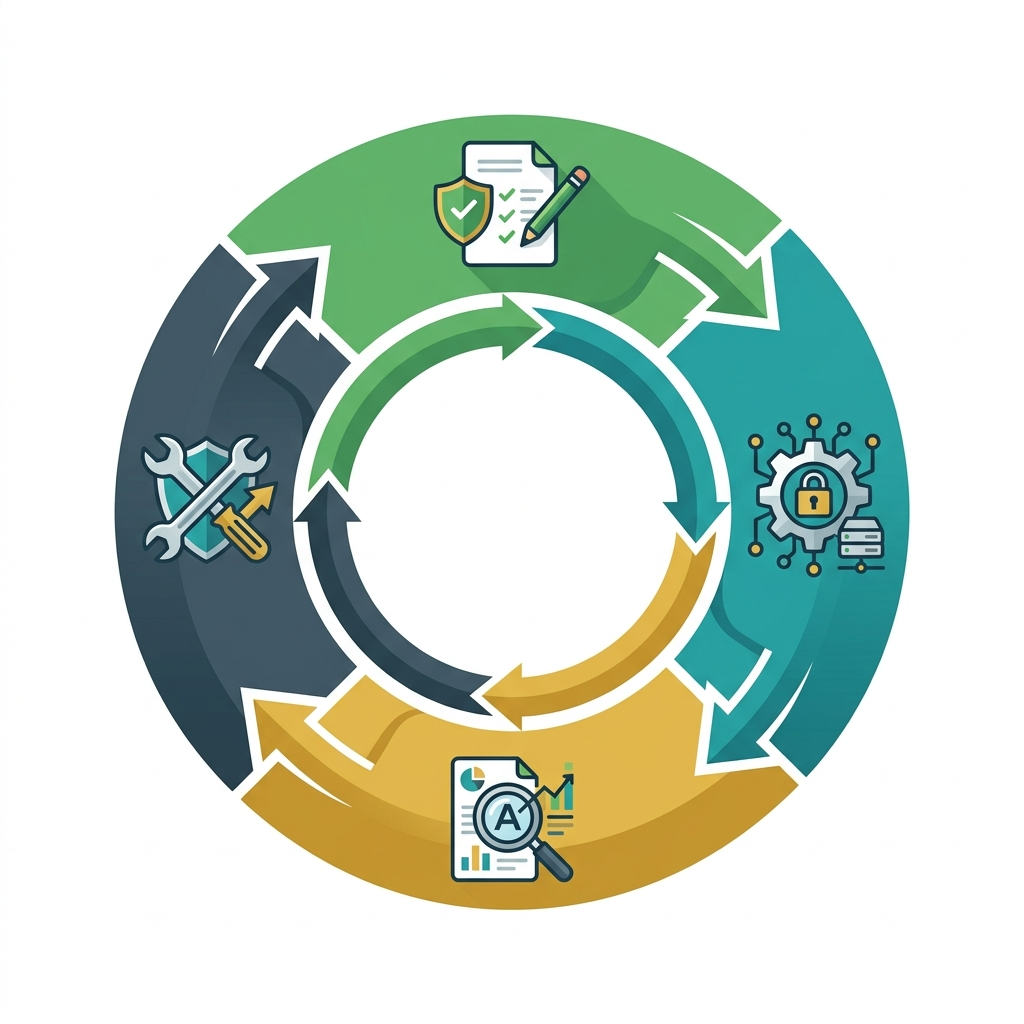
\includegraphics[width=0.95\textwidth]{pdca_cycle.png}
    \end{column}
  \end{columns}
  % Nota: Para que la solución sea sostenible, se alinea con la ISO 27001 mediante el ciclo PDCA, garantizando auditoría interna y mejoras reactivas y preventivas permanentes.
\end{frame}

\section{Conclusiones y Referencias}
\subsection{Conclusiones y Referencias}

% 11. Conclusiones
\begin{frame}{Conclusiones y Lecciones Clave}
  \begin{itemize}
    \item   \textbf{Seguridad de IA Holística}: Asegurar sistemas inteligentes exige blindar tanto las APIs de red clásicas como la integridad matemática del clasificador.
    \item   \textbf{Resiliencia Proactiva}: El suavizado espectral y rollbacks en caliente en menos de 5 segundos conmutan de forma segura ante intrusiones complejas de evasión.
    \item   \textbf{Consistencia de Integridad}: La formalización del modelo de Biba sobre el control ABAC previene contaminaciones de datos de baja confianza.
    \item   \textbf{Auditoría y Estándares}: La alineación con NIST AI RMF, MITRE ATLAS e ISO 27001 otorga un marco de cumplimiento técnico-administrativo corporativo.
  \end{itemize}
  % Nota: En conclusión, SentinelML-ABAC propone una arquitectura robusta que combina ciberseguridad clásica y MLSecOps para proteger infraestructuras críticas contra atacantes APTs.
\end{frame}

% 12. Referencias
\begin{frame}{Referencias Bibliográficas}
  \begin{block}{Estándares y Literatura Científica}
    \footnotesize
    \begin{thebibliography}{9}
      \setbeamertemplate{bibliography item}[text]
      \bibitem{nist800} NIST. (2018). \textit{NIST SP 800-53, Rev. 5: Security and Privacy Controls}.
      \bibitem{iso27001} ISO/IEC. (2022). \textit{ISO/IEC 27001:2022: Information Security Management Systems}.
      \bibitem{goodfellow2014} Goodfellow, I. J., et al. (2014). \textit{Explaining and harnessing adversarial examples}. arXiv:1412.6572.
      \bibitem{nistairmf} NIST. (2023). \textit{Artificial Intelligence Risk Management Framework (AI RMF 1.0)}.
    \end{thebibliography}
  \end{block}
  % Nota: Estas son algunas de las referencias principales utilizadas para fundamentar y verificar el sustento científico de nuestra solución. Muchas gracias por su atención.
\end{frame}

\end{document}
